\documentclass[11pt]{jarticle}

\usepackage[dvipdfmx]{graphicx}
\usepackage{sty/fancyheadings}
\usepackage{sty/sotsuron2009}
\usepackage{here}
\usepackage{ascmac}
\usepackage[subrefformat=parens]{subcaption}
\usepackage{here}
\usepackage{cite}
\usepackage{amsmath}
\pagestyle{empty}
\usepackage{bm}
\usepackage{comment}
\linesparpage{40}
%\makeatletter
%\renewcommand{\theequation}{
%\thesection.\arabic{equation}}
%\@addtoreset{equation}{section}
%\makeatother
\pagestyle{fancy}

\newcommand{\argmin}{\mathop{\rm arg~min}\limits}

\begin{document}

\begin{comment}
\title{
 \LARGE
 % 卒論和文タイトル
 \\ \\
 \large
 % 卒論英文タイトル
}

\author{
 研究者 高専 太郎\\
 指導教員 中西 大輔\\ \\
 松江工業高等専門学校\\
 電子制御工学科\\ \\
}

\date{平成29年2月13日}

\maketitle
\end{comment}

\thispagestyle{empty}
\newpage
\section*{概要}
        % 概要

\thispagestyle{empty}
\newpage
\tableofcontents
\thispagestyle{empty}

%章ごとに呼び出し

\newpage
\setcounter{page}{1}
\section{緒言}
    % 緒言
\newpage
\section{空気圧人工筋肉}
\subsection{McKibben型空気圧人工筋肉アクチュエータ(MPA)}
MPAはシリコンゴムチューブをナイロンメッシュで覆うことで構成されており(図\ref{fig:MPA}\subref{fig:Structure}),両端に栓をするシンプルな構造である.
これに圧縮した空気を印加することでシリコンゴムチューブが膨張しメッシュによる自身の軸方向への張力が発生するアクチュエータである\cite{Yu22}(図\ref{fig:MPA}\subref{fig:move}).
高出力かつ素材自体も軽量で,物理的柔軟性による高い弾性力を持つという利点があり,筋肉の代用として生物を模したロボットやリハビリなどに用いられる.
図1に示すような直径が数10 mmのものが一般的であるが,近年では直径数 mm程度の細径タイプのMPAも普及している\cite{7989580}.細径化することで集積することが可能となり複雑な筋肉などにも
応用がされている.しかしさらなる高集積化,小動物や昆虫型などの小型なロボットへの応用を考える上ではより細径な人工筋肉の開発が求められている.しかし,現在細径MPAは最も細いもので3 mm(韓国サムスン電子グループ)
であり,また自作する場合でもナイロンメッシュは3mm程度のものが最細である.またメッシュの製作には製紐機(ブレーダー)と呼ばれる特殊な機械が必要であり,研究室で内製することは困難である.
すなわち,McKibben方式でこれ以上細径な空圧筋を作ることは困難である
%%%%%%%%%%%%%%%%%%%%%%%%%%%%%%%%%%%%%%%%%%%%%%%%%%%%%%%%%
\begin{figure}[ht]
    %
    \begin{minipage}{0.49\columnwidth}
      \vspace{4mm}
      \centering
      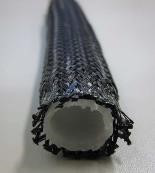
\includegraphics[scale=1]{pic/MPA_kousei.png}
      \vspace{3mm}
      \subcaption{MPA断面図}
      \label{fig:Structure}
    \end{minipage}
    %
    \begin{minipage}{0.49\columnwidth}
      \vspace{25mm}
      \centering
      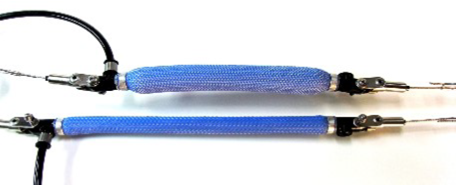
\includegraphics[scale=0.8]{pic/MPA_dousa.png}
      \subcaption{MPA外観および動作の様子}
      \label{fig:move}
    \end{minipage}
    %
    \caption{McKibben型空気圧人工筋(MPA)の構成および外観\cite{中西大輔2020}}
    \label{fig:MPA}
  \end{figure}.
\newpage
\subsection{軸方向繊維強化型人工筋肉}
そこで本研究ではMcKibbenタイプではなく,軸方向遷移強
化型の空圧筋\cite{}に着目する.軸方向繊維強化型人工筋肉の動作原理を図\ref{fig:siku}に示す.
この人工筋肉は,ゴムチューブ内に拘束繊維を内包する構造で,拘束繊維とゴムチューブとの摩耗を抑え長寿命を実現する.
空気圧が供給されると,内圧が半径方向にのみ伝達され,軸方向への効率的な収縮を引き起こす.
さらに,チューブに外挿されたリングの数を調整することで,ゴムチューブの膨張を抑制しつつ必要な収縮力を発揮できる\cite{3}
McKibbenタイプに比べ比較的構造が簡単であり市販されているナイロンメッシュの細さに細径化が左右されないためこの方式での研究を行った.
\begin{figure}[h]
  \centering  % 図全体を中央に配置
  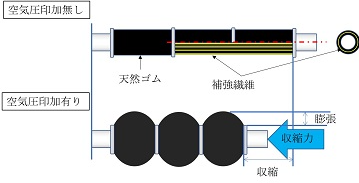
\includegraphics[scale=1]{pic/A.PNG}
  \caption{軸方向繊維強化型人工筋肉の仕組み\cite{4}}
  \label{fig:siku}
\end{figure}


            % 本文
% 必要に応じて章を増やす,またファイル名もsec2, sec3である必要はない
% このmain.texが置いてあるディレクトリ内にある「chapters」フォルダ以下に
% 自分がわかりやすい名前のtexファイルを作成し,\include{chapters/*****}で
% 呼び出せば良い
\newpage
\section{結言}

本研究では,ゴム皮膜を用いた軸方向繊維強化型人工筋肉による,超細径空気圧人工筋肉の開発を目的として研究を行った.
まず液体ゴムを用いて細径風船の作製を行い,凝固液の適切な乾かし方,液体ゴムに浸す時間についての知見を得た.
その後最適なゴムと水の割合,ムラのできない作製方法の確立を行った.次に内径5 mmの人工筋肉の作製を行いゴム被膜に糸を内包するノウハウを得た.
そのノウハウを生かして様々な作製方法を模索し,内径3 mmの人工筋肉の作製に成功した.最後に評価実験を行い,収縮率が9.3 \%,発揮張力が138.4 gであることが確認でき,空圧筋として動作した.
\noindent

今後はより細径な軸方向繊維強化型人工筋肉を目指すとともに性能の向上に取り組む予定である.
      % 結言
\newpage
\section{謝辞} % 謝辞
% できればbibtexを使ってください

\newpage
\bibliographystyle{junsrt}
\bibliography{sanko.bib}


    % 参考文献

\end{document}
